%version revue NS
\documentclass[a4paper,11pt]{report}
\usepackage[showexo=true,showcorr=false]{../packages/coursclasse}
\usepackage{pgfplots}
\pgfplotsset{compat=1.15}
\usepackage{mathrsfs}
\usetikzlibrary{arrows}
\toggletrue{montrerNiveaux}
%permet de gérer l'espacement entre les items des env enumerate et enumitem
\usepackage{enumitem}
\setlist[enumerate]{align=left,leftmargin=1cm,itemsep=10pt,parsep=0pt,topsep=0pt,rightmargin=0.5cm}
\setlist[itemize]{align=left,labelsep=1em,leftmargin=*,itemsep=0pt,parsep=0pt,topsep=0pt,rightmargin=0cm}
%permet de gerer l'espacement entre les colonnes de multicols
\setlength\columnsep{20pt}

% \usepackage{pst-circ,pstricks-add}
% \usepackage{psfrag}
% \usepackage{pst-eucl}
% \usepackage{pst-all}
% \usepackage[pspdf={-dNOSAFER -dALLOWPSTRANSPARENCY}]{auto-pst-pdf}
\begin{document}


%%%%%%%%%%%%%%%%% À MODIFIER POUR CHAQUE SERIE %%%%%%%%%%%%%%%%%%%%%%%%%%%%%
\newcommand{\chapterName}{Espace}
\newcommand{\serieName}{Cercles, lieux géométriques}


%%%%%%%%%%%%%%%%%% PREMIERE PAGE NE PAS MODIFER %%%%%%%%%%%%%%%%%%%%%%%%
% le chapitre en cours, ne pas changer au cours d'une série
\chapter*{\chapterName}
\thispagestyle{empty}

%%%%% LISTE AIDE MEMOIRE %%%%%%
\begin{amL}{\serieName}{
\item Droites sécantes (page 92)
\item Droites perpendiculaires (page 93)
\item Droites parallèles (page 94)
\item Médiatrice d'un segment (page 96)
\item Cercle et disque (page 99)
\item Arc de cercle et secteur circulaire (page 100)
\item Angle (page 101)
\item Bissectrice d'un angle (page 105)
}
\end{amL}

%%%%%%%%%%%%%%% DEBUT DE LA SERIE NE PAS MODIFIER %%%%%%%%%%%%%%%%%%%%%%%%%%%%%
\section*{\serieName}
\setcounter{page}{1}
\thispagestyle{firstPage}



%%%%%%%%%%% LES EXERCICES %%%%%%%%%%%%%%%%%%%%%%%%%%%%%%%%%%%%

\begin{resolu}{Concstruction de cercles}{
\begin{minipage}[t]{0.6\textwidth}{
\vspace{0pt}
Trace les cercles suivants:
\begin{tasks}[after-item-skip = 0.4em]
    \task Trace le cercle $C1$ de centre $A$ et de rayon $r$.
    \task[]Solution: Commence par reporter la longueur $r$ à l'aide de ton compas. Puis sans changer l'écartement, pique sur le point $A$ et trace le cercle de rayon $r$. 
    \task Trace le cercle $C2$ de centre $A$ passant par $B$.
    \task[]Solution: Pique ton compas sur le point $A$ puis pose la mine du compas sur le point $B$. Trace ensuite le cercle. 
\end{tasks}
}
\end{minipage}
\begin{minipage}[t]{0.4\textwidth}{
\vspace{0pt}
\begin{center}	
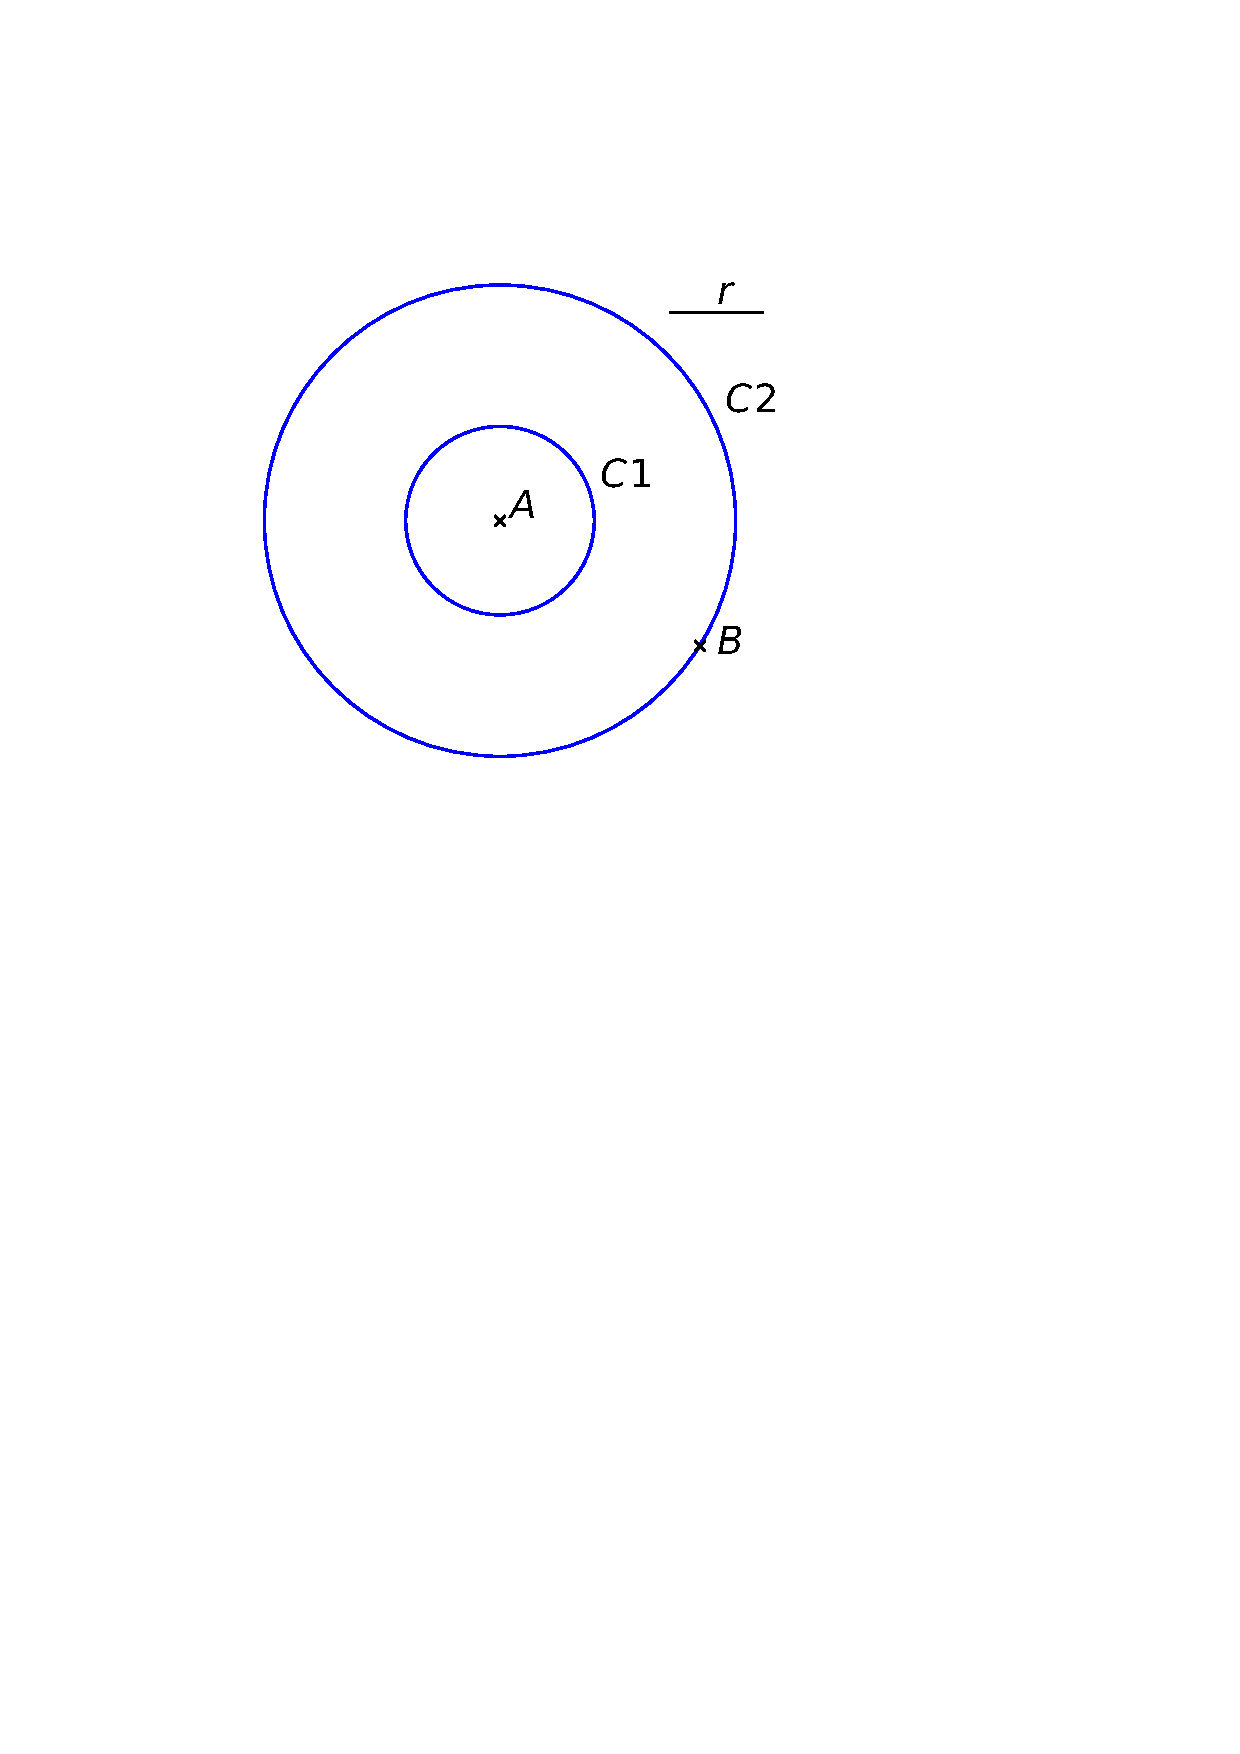
\includegraphics[scale=0.6]{media/es-10/12-1-b}
\end{center}
}
\end{minipage}
%\psset{xunit=1cm,yunit=1cm,algebraic=true,dimen=middle,dotstyle=o,dotsize=5pt 0,linewidth=2pt,arrowsize=3pt 2,arrowinset=0.25}
%\begin{pspicture*}(-9.48,-5.06)(2.64,5.26)
%\pscircle[linewidth=2pt](-4,0){2}
%\pscircle[linewidth=2pt](-4,0){5}
%\begin{scriptsize}
%\psdots[dotstyle=x](-4,0)
%\rput[bl](-3.92,0.2){$A$}
%\psdots[dotstyle=x](-1,-4)
%\rput[bl](-1.1,-3.8){$B$}
%\rput[bl](-5.02,1.3){$C1$}
%\rput[bl](-6.52,3.86){$C2$}
%\end{scriptsize}
%\end{pspicture*}
}
{1}
\end{resolu}


\begin{exop}
{Effectue les constructions suivantes (sur la page d'après):
\begin{tasks}[after-item-skip = 0.3em](1)
    \task Construis le cercle $C1$ de centre $B$ et de rayon $[AB]$.
    \task Construis le cercle $C2$ de centre $E$ et de rayon \tunit{2}{\cm}.
    \task Construis le cercle $C3$ de centre $E$ passant par $F$.
    \task Construis le cercle $C4$ de diamètre $CD$, passant par $C$ et $D$.
\end{tasks}
\begin{center}	
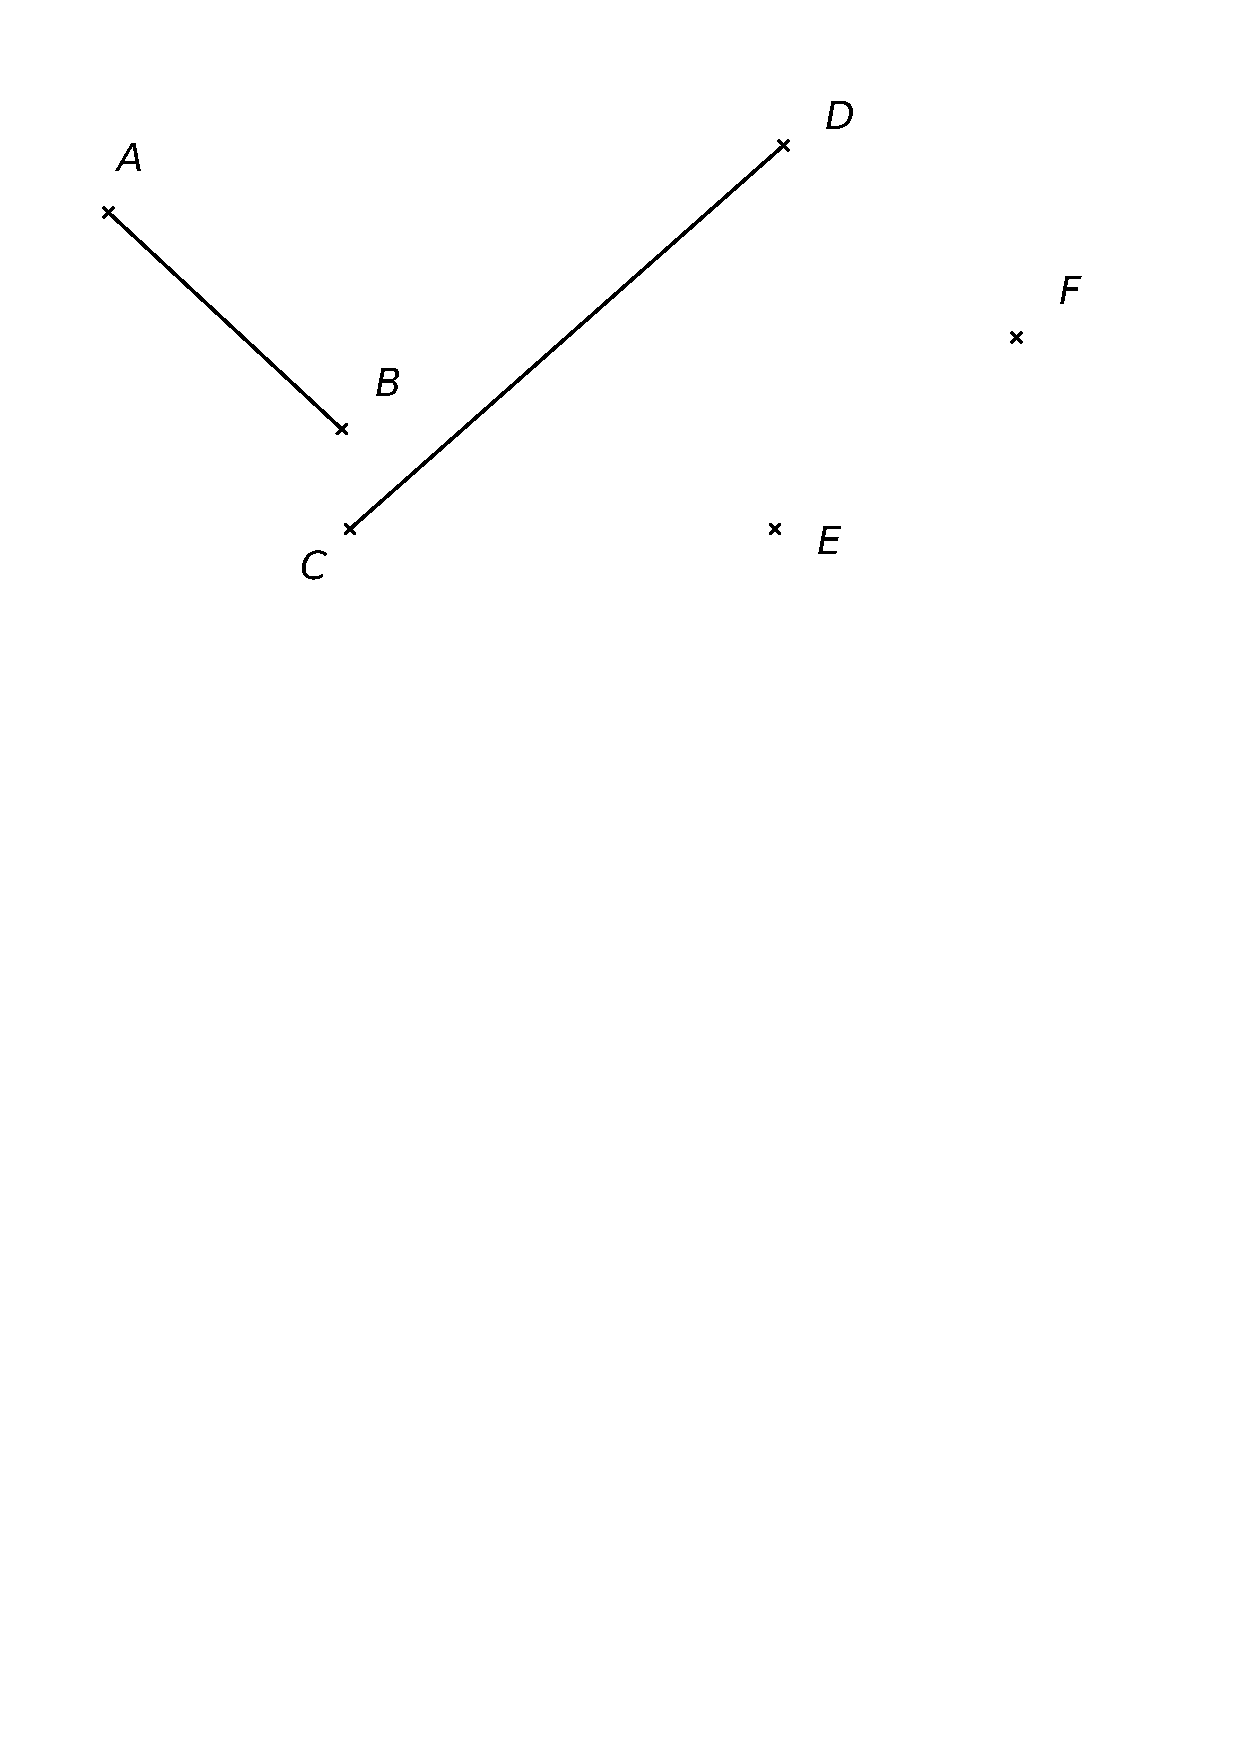
\includegraphics[scale=0.8]{media/es-10/12-2}
\end{center}
%\begin{center}
%\psset{xunit=1cm,yunit=1cm,algebraic=true,dimen=middle,dotstyle=o,dotsize=5pt 0,linewidth=2pt,arrowsize=3pt 2,arrowinset=0.25}
%\begin{pspicture*}(-8.16,-5)(6.98,2.66)
%\psline[linewidth=2pt](-7.8,1.54)(-4.6,-0.68)
%\psline[linewidth=2pt](0.3,1.48)(-4.14,-3.68)
%\begin{scriptsize}
%\psdots[dotstyle=x](-7.8,1.54)
%\rput[bl](-7.72,1.74){$A$}
%\psdots[dotstyle=x](-4.6,-0.68)
%\rput[bl](-4.52,-0.48){$B$}
%\psdots[dotstyle=x](-4.14,-3.68)
%\rput[bl](-4.2,-3.48){$C$}
%\psdots[dotstyle=x](0.3,1.48)
%\rput[bl](0.38,1.68){$D$}
%\psdots[dotstyle=x](1.42,-4.1)
%\rput[bl](1.5,-3.9){$E$}
%\psdots[dotstyle=x](5.74,0.54)
%\rput[bl](5.82,0.74){$F$}
%\end{scriptsize}
%\end{pspicture*}
%\end{center}
}
{1}
\end{exop}

\begin{exo}
{Effectue les constructions suivantes:
\begin{tasks}(1)
	\task Trace un segment $[AB]$ de \tunit{3}{\cm}.
	\task Trace le cercle de centre $A$ et de rayon \tunit{2}{\cm}.
    \task Trace le cercle de centre $B$ et de rayon $[AB]$.
\end{tasks}
}
{1}
\end{exo}

\begin{exo}
{Effectue les constructions suivantes:
\begin{tasks}(1)
	\task Trace un cercle de centre $O$ et de rayon \tunit{3}{\cm}.
    \task Place un point $A$ sur le cercle. Trace une corde $[AB]$ tels que  $[AB]$=\tunit{6}{\cm}.
\end{tasks}
Quel est le nom de cette corde~? 
}
{2}
\end{exo}

\begin{exol}{ES21}{99}{1}
\end{exol}


\begin{exo}
{Un cheval est attaché à un poteau $P$ dans un champ. Sa corde mesure 3 mètres. En utilisant une échelle de 1:100 (1 mètre en réalité correspond à 1 centimètre sur la carte), trace la zone dans laquelle le cheval peut se promener.

%\psset{xunit=1cm,yunit=1cm,algebraic=true,dimen=middle,dotstyle=o,dotsize=5pt 0,linewidth=2pt,arrowsize=3pt 2,arrowinset=0.25}
%\begin{pspicture*}(-3.63,-6.08)(9.99,1.44)
%\begin{scriptsize}
%\psdots[dotstyle=x](2.67,-2.76)
%\rput[bl](2.75,-2.56){$P$}
%\end{scriptsize}
%\end{pspicture*}
}
{1}
\end{exo}

\begin{exol}{ES22}{99}{1}
\end{exol}

\begin{exop}
{
	Place le point $P$ à $\tunit{3}{cm}$ du point $A$ et à \tunit{2}{cm} de la droite $d$.

\begin{center}	
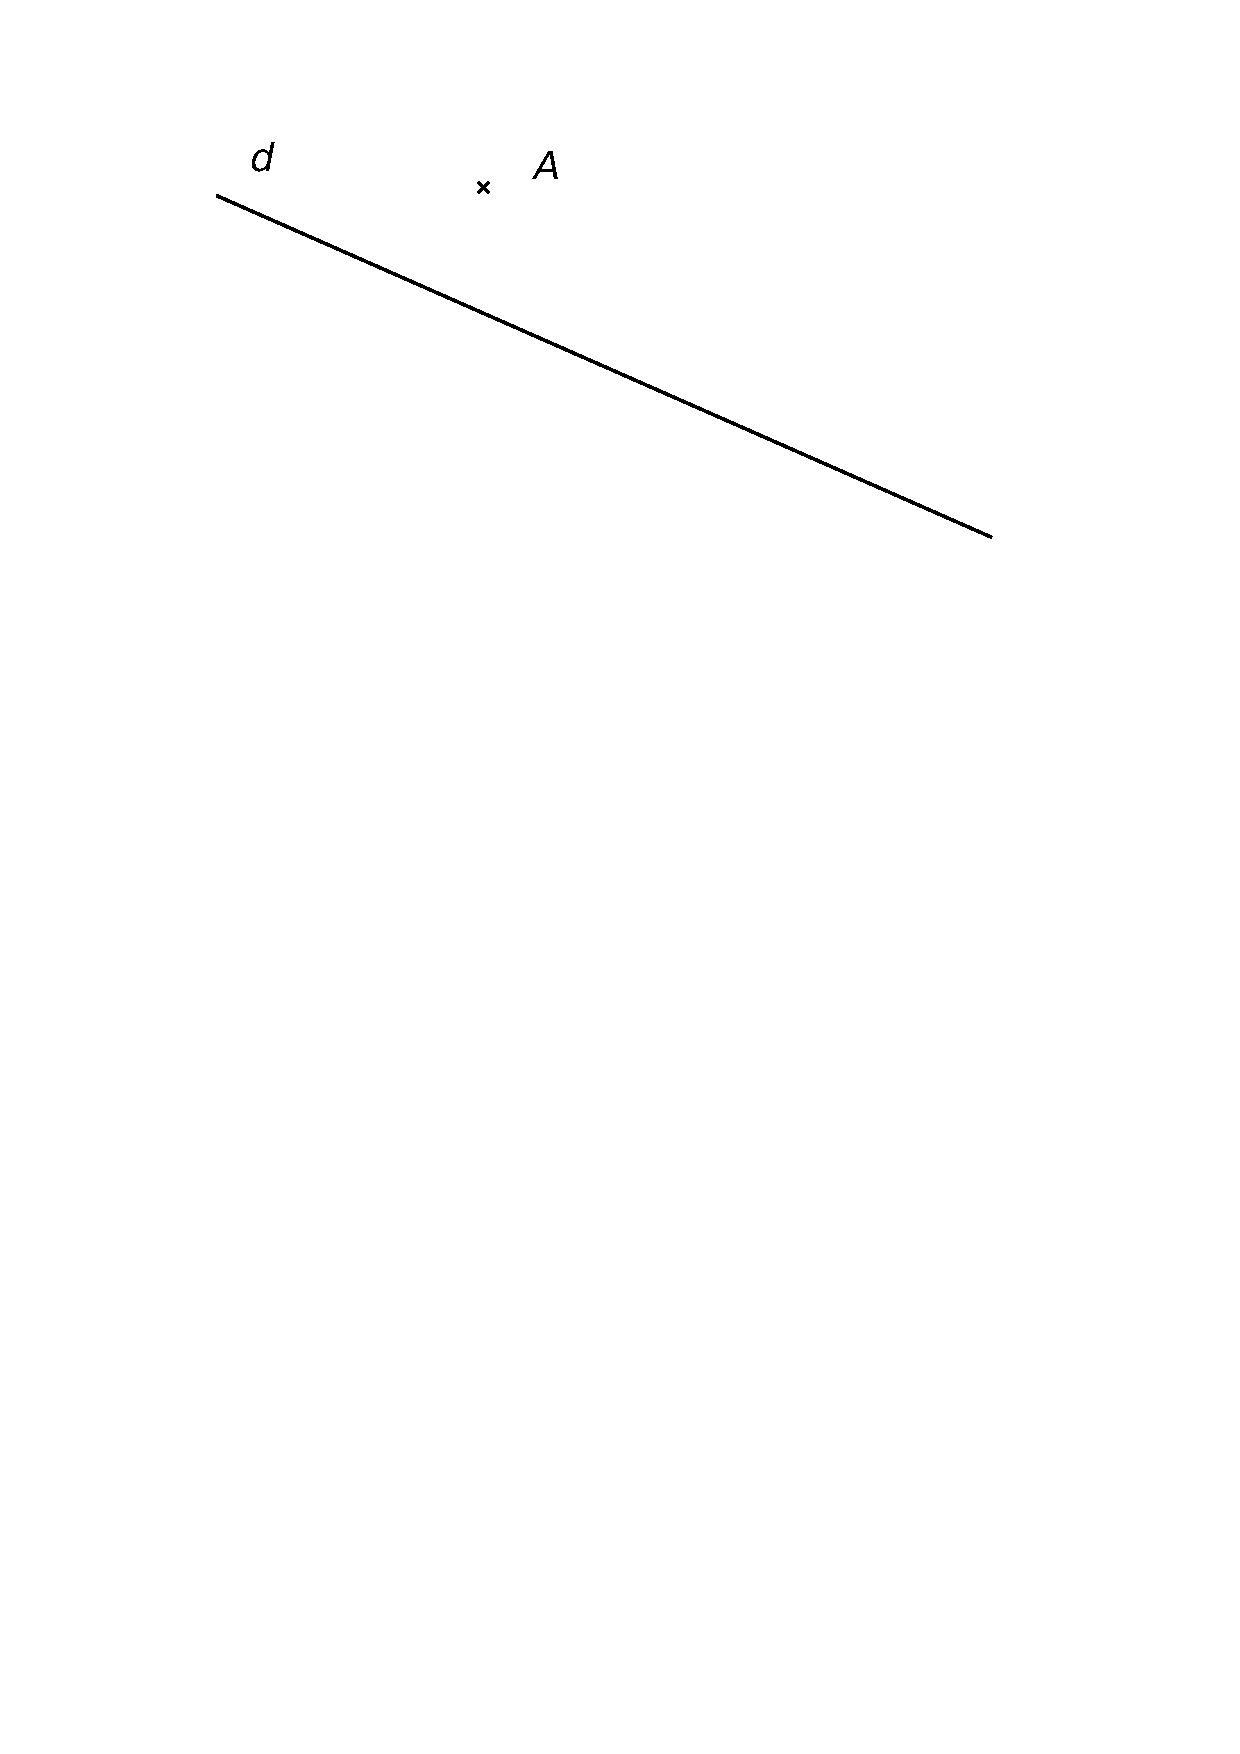
\includegraphics[scale=0.8]{media/es-10/12-3}
\end{center}
%\psset{xunit=1cm,yunit=1cm,algebraic=true,dimen=middle,dotstyle=o,dotsize=5pt 0,linewidth=2pt,arrowsize=3pt 2,arrowinset=0.25}
%\begin{pspicture*}(-3.63,-4.22)(9.99,1.3)
%\psplot[linewidth=2pt]{-3.63}{9.99}{(-14.5524-1.48*x)/9.5}
%\begin{scriptsize}
%\rput[bl](-2.87,-0.8){$d$}
%\psdots[dotstyle=x](-0.91,-0.7)
%\rput[bl](-0.83,-0.5){$A$}
%\end{scriptsize}
%\end{pspicture*}
\vspace{-0.7cm}
}
{1}
\end{exop}

\begin{resolu}{Reconnaître une médiatrices}{Laquelle de ces trois droites est plus vraisemblablement une médiatrice du segment $[AB]$~?
%\psset{xunit=1cm,yunit=1cm,algebraic=true,dimen=middle,dotstyle=o,dotsize=5pt 0,linewidth=2pt,arrowsize=3pt 2,arrowinset=0.25}
%\begin{pspicture*}(-1.33,-4.1)(12.29,1.42)
%\psline[linewidth=2pt](-0.91,-0.7)(2.09,-0.68)
%\psplot[linewidth=2pt]{-1.33}{12.29}{(--0.1024--3*x)/-0.02}
%\psline[linewidth=2pt](3.33,-0.68)(6.65,-0.66)
%\psplot[linewidth=2pt]{-1.33}{12.29}{(-16.5534--3.32*x)/-0.02}
%\psline[linewidth=2pt](7.91,-0.66)(10.93,-0.68)
%\psplot[linewidth=2pt]{-1.33}{12.29}{(--11.1739-1.13*x)/-0.79}
%\begin{scriptsize}
%\psdots[dotstyle=x](-0.91,-0.7)
%\rput[bl](-0.83,-0.5){$A$}
%\psdots[dotstyle=x](2.09,-0.68)
%\rput[bl](2.17,-0.48){$B$}
%\rput[bl](0.11,0.94){$g$}
%\psdots[dotstyle=x](3.33,-0.68)
%\rput[bl](3.41,-0.48){$D$}
%\psdots[dotstyle=x](6.65,-0.66)
%\rput[bl](6.73,-0.46){$E$}
%\rput[bl](5.13,0.94){$i$}
%\psdots[dotstyle=x](7.91,-0.66)
%\rput[bl](7.99,-0.46){$G$}
%\psdots[dotstyle=x](10.93,-0.68)
%\rput[bl](11.01,-0.48){$H$}
%\rput[bl](7.31,-3.94){$k$}
%\end{scriptsize}
%\end{pspicture*}

\vspace{-0.8cm}
\begin{center}	
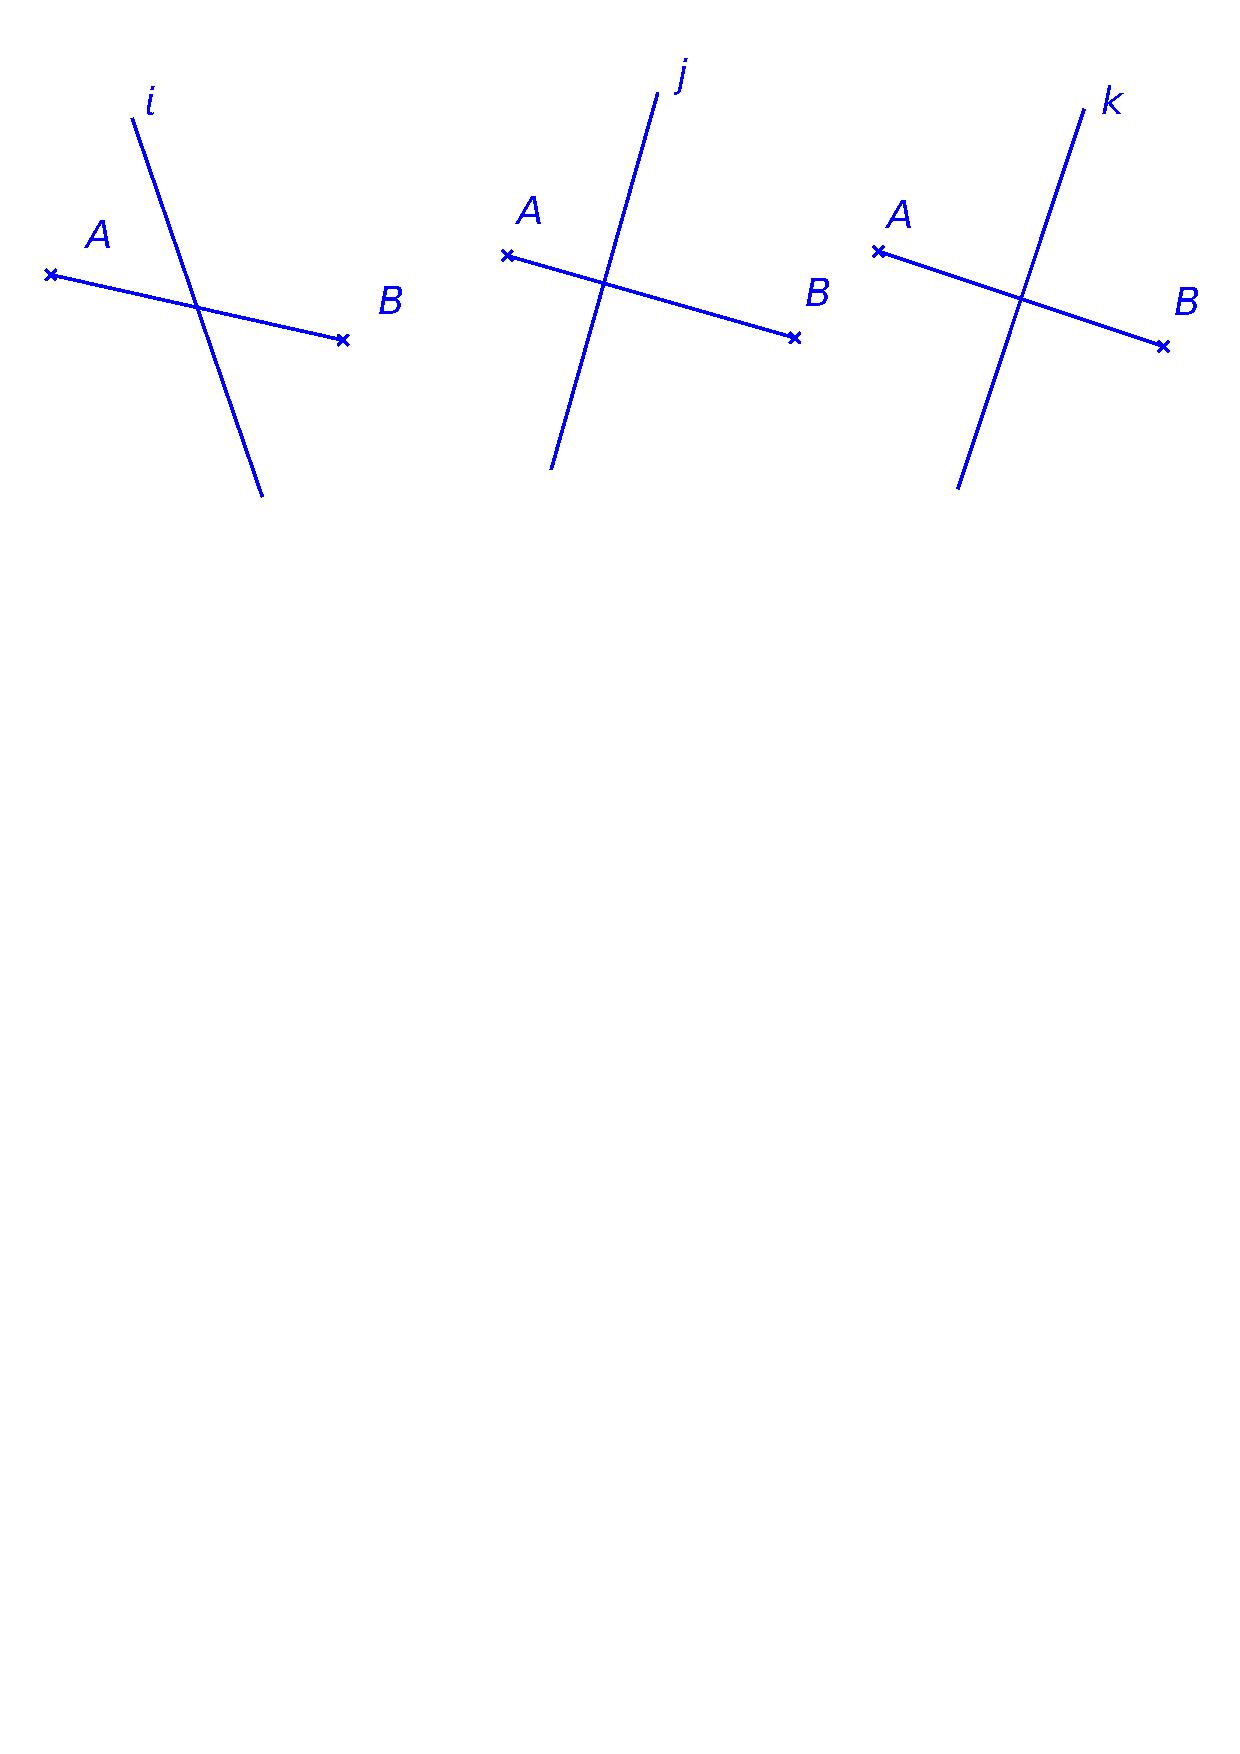
\includegraphics[scale=0.5]{media/es-10/12-5}
\end{center}
\vspace{-2cm}
La droite $j$, car elle est perpendiculaire au segment $[AB]$ et passe par son milieu. La droite $i$ ne passe pas par le milieu de $[AB]$ et la droite $k$ n'est pas perpendiculaire au segment $[AB]$.
}
{1}
\end{resolu}


\begin{exop}
	{Parmi les droites suivantes, lesquelles sont des médiatrices du segment $[AB]$~?    Justifie ta réponse.
\begin{center}	
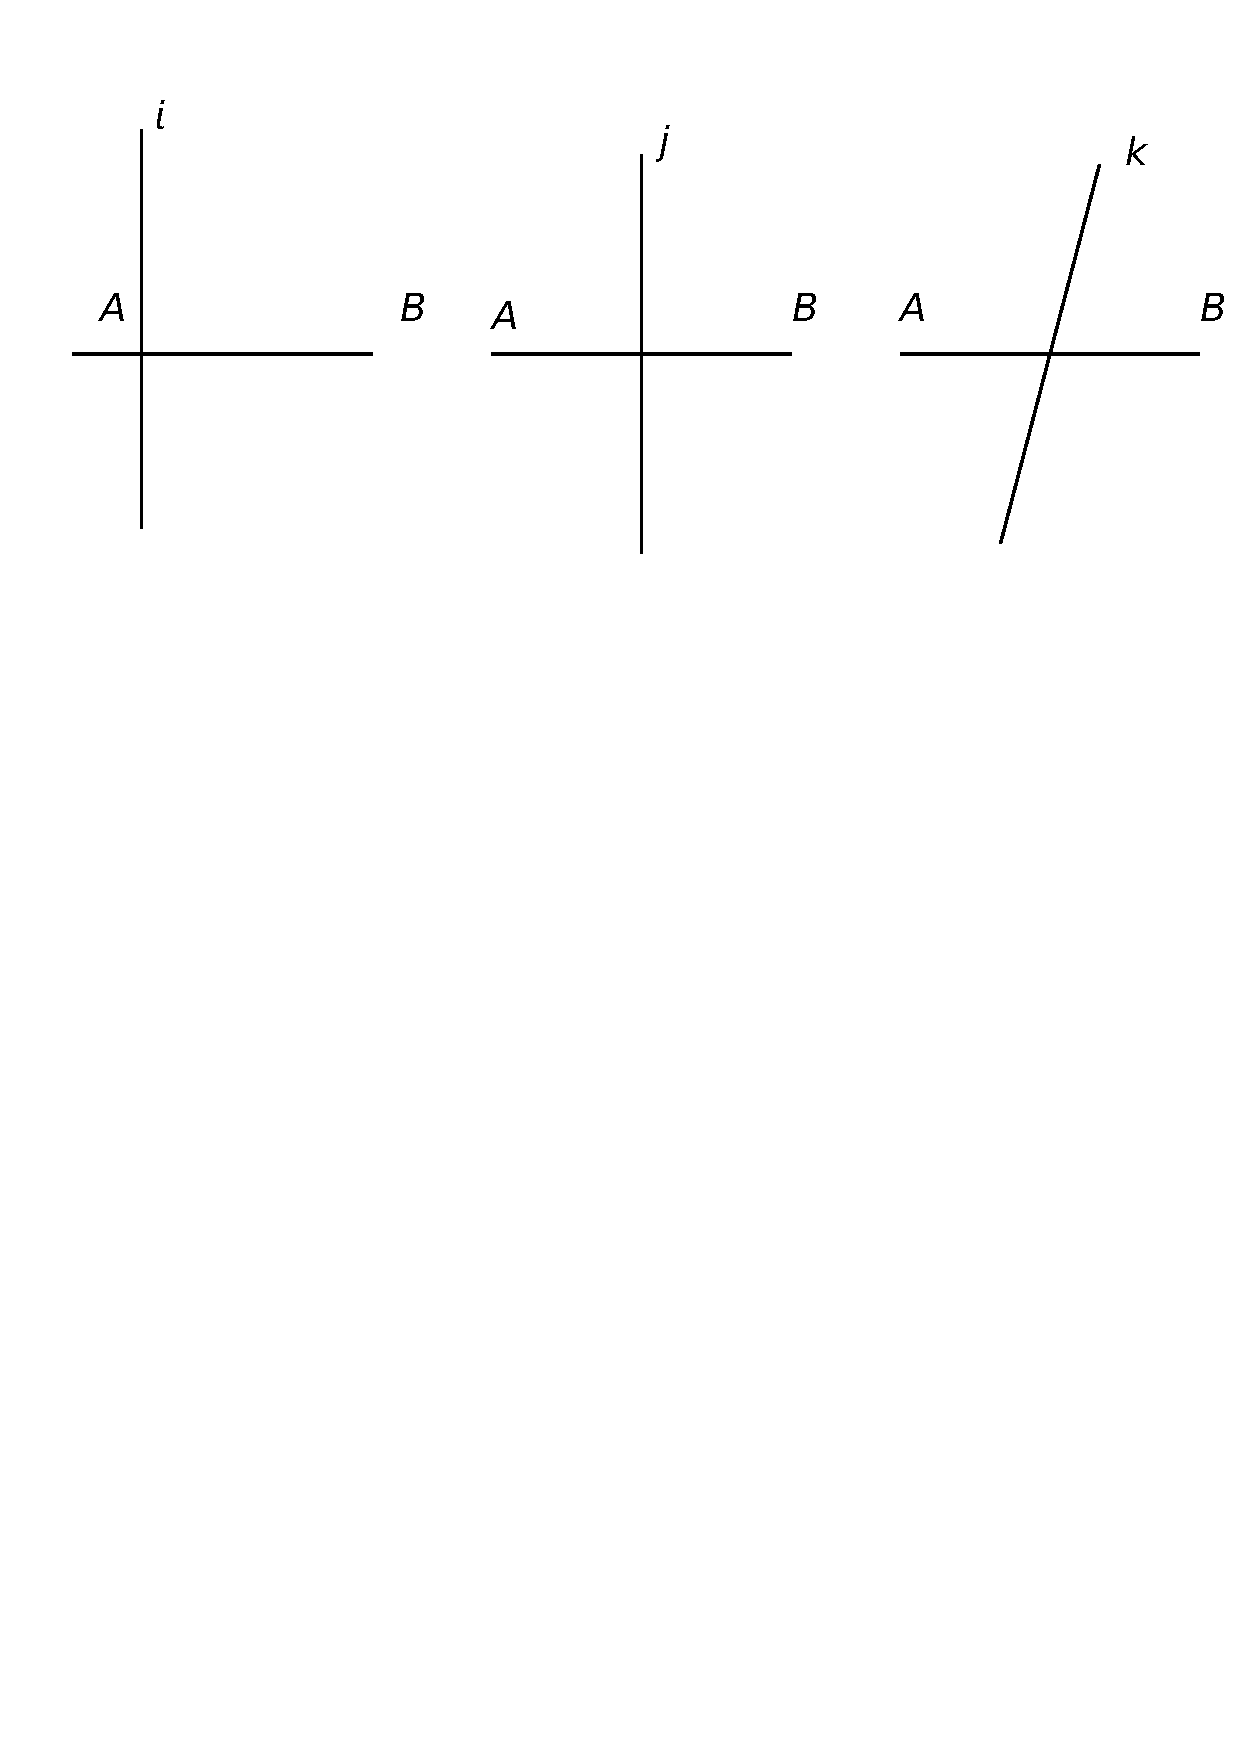
\includegraphics[scale=0.8]{media/es-10/12-4}
\end{center}
   \begin{tasks}(1)
      \task[$i$:] \hrulefill  
      \task[$j$:] \hrulefill 
       \task[$k$:] \hrulefill
\end{tasks}
  \vspace{1cm}
  \begin{center}
%\psset{xunit=1cm,yunit=1cm,algebraic=true,dimen=middle,dotstyle=o,dotsize=5pt 0,linewidth=2pt,arrowsize=3pt 2,arrowinset=0.25}
%\begin{pspicture*}(-4.27,-6.57)(10.87,1.09)
%\psline[linewidth=2pt](-3.69,-2.33)(-0.45,-1.51)
%\psline[linewidth=2pt](-0.83,-4.77)(3.71,-2.89)
%\psline[linewidth=2pt](4.33,-1.35)(8.61,-2.65)
%\psplot[linewidth=2pt]{-4.27}{10.87}{(--8.2812--3.24*x)/-0.82}
%\psplot[linewidth=2pt]{-4.27}{10.87}{(--10.3512-4.24*x)/-1.12}
%\psplot[linewidth=2pt]{-4.27}{10.87}{(-35.745--4.28*x)/1.3}
%\begin{scriptsize}
%\psdots[dotstyle=x](-3.69,-2.33)
%\rput[bl](-3.61,-2.13){$A$}
%\psdots[dotstyle=x](-0.45,-1.51)
%\rput[bl](-0.37,-1.31){$B$}
%\psdots[dotstyle=x](-0.83,-4.77)
%\rput[bl](-0.75,-4.57){$C$}
%\psdots[dotstyle=x](3.71,-2.89)
%\rput[bl](3.79,-2.69){$D$}
%\psdots[dotstyle=x](4.33,-1.35)
%\rput[bl](4.41,-1.15){$E$}
%\psdots[dotstyle=x](8.61,-2.65)
%\rput[bl](8.69,-2.45){$F$}
%\rput[bl](-2.41,0.19){$d1$}
%\rput[bl](2.55,-0.67){$d2$}
%\rput[bl](7.85,0.17){$d3$}
%\end{scriptsize}
%\end{pspicture*}  
 \end{center}

} 
{1}
\end{exop}

\begin{exol}{ES34}{101}{2}
\end{exol}


\begin{exop}
{
À l'aide de la règle et de l'équerre, trace les médiatrices de ces segments.
\begin{center}
	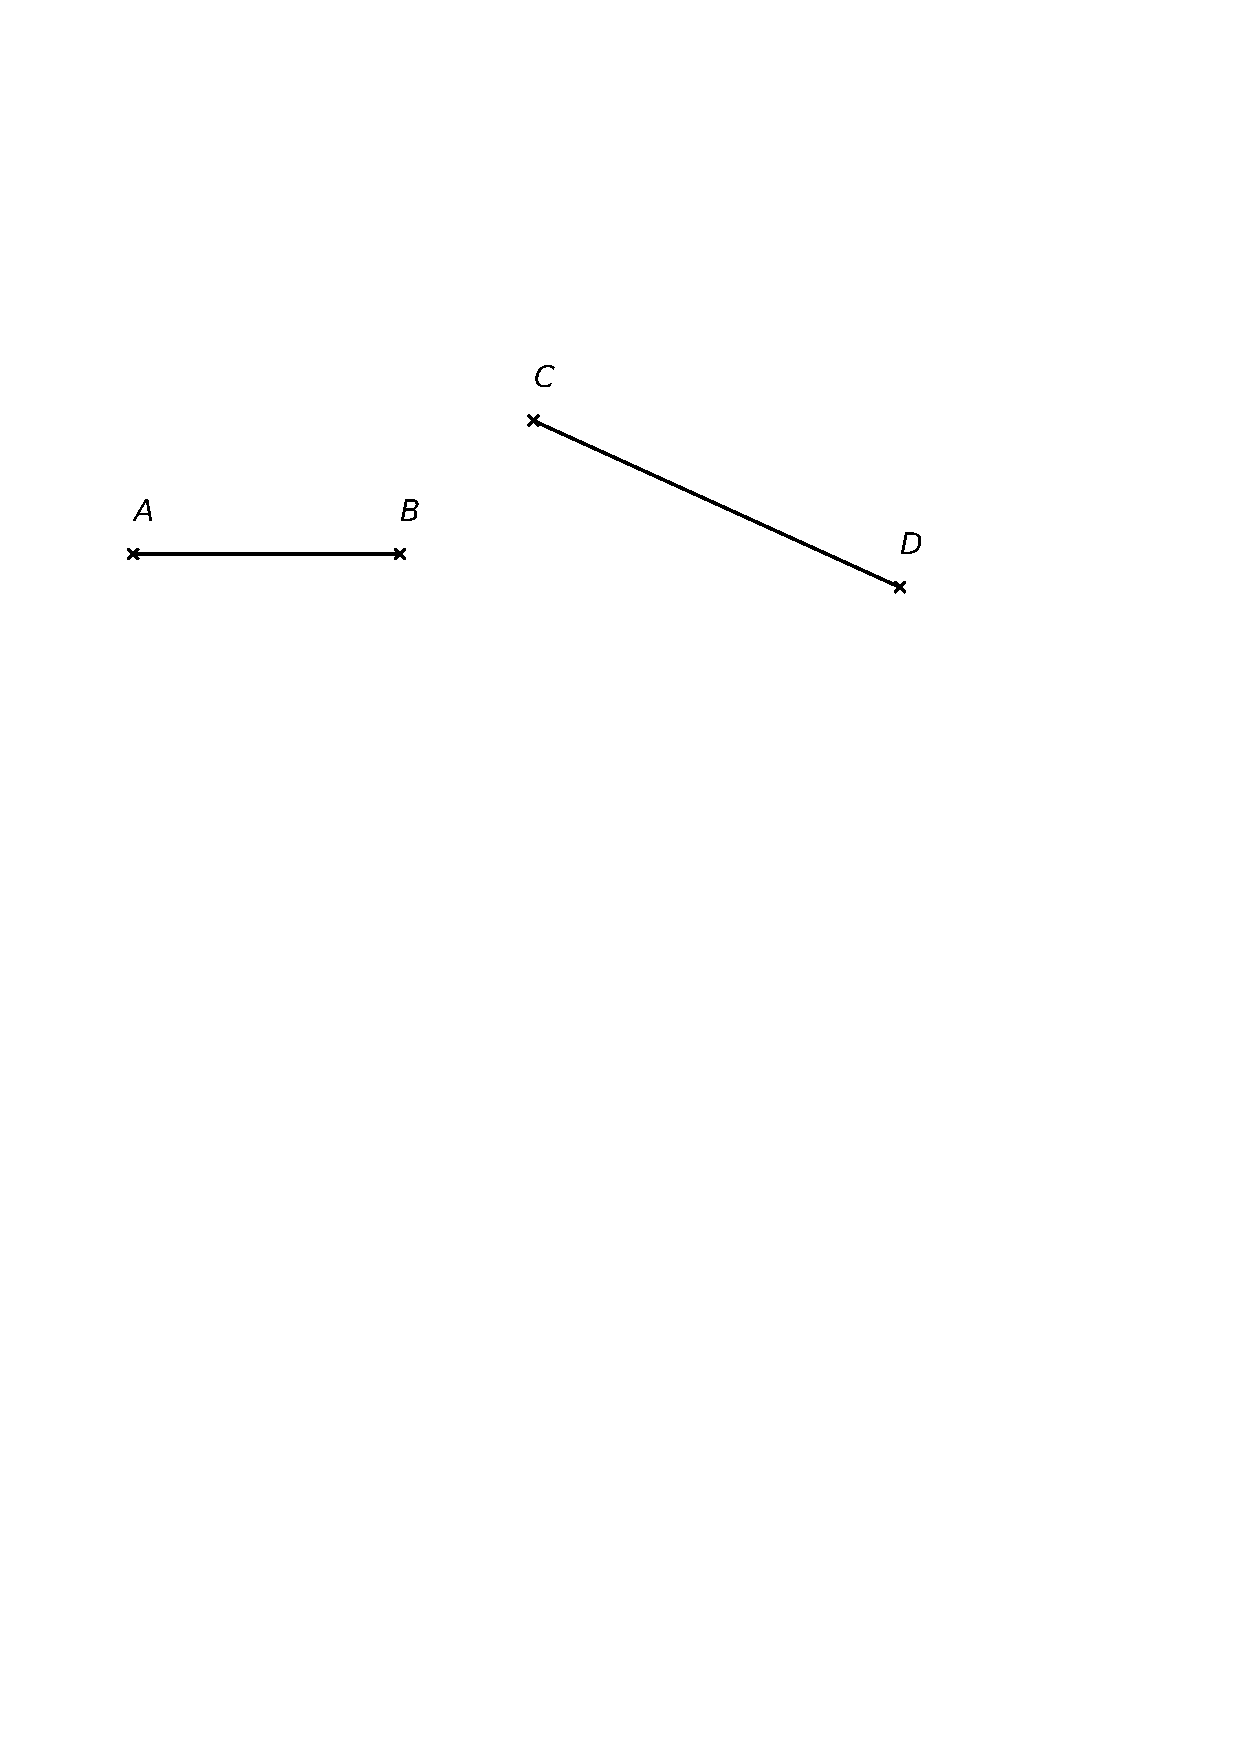
\includegraphics[scale=1]{media/es-10/12-7}
\end{center}
\vspace{2cm}
%\begin{center}
%\psset{xunit=1cm,yunit=1cm,algebraic=true,dimen=middle,dotstyle=o,dotsize=5pt 0,linewidth=2pt,arrowsize=3pt 2,arrowinset=0.25}
%\begin{pspicture*}(-4.27,-3.45)(19.29,-0.57)
%\psline[linewidth=2pt](-2.65,-2.25)(0.35,-2.25)
%\psline[linewidth=2pt](2.13,-1.21)(8.13,-3.21)
%
%\begin{scriptsize}
%\psdots[dotstyle=x](-2.65,-2.25)
%\rput[bl](-2.57,-2.05){$A$}
%\psdots[dotstyle=x](0.35,-2.25)
%\rput[bl](0.43,-2.05){$B$}
%\psdots[dotstyle=x](2.13,-1.21)
%\rput[bl](2.21,-1.01){$C$}
%\psdots[dotstyle=x](8.13,-3.21)
%\rput[bl](8.21,-3.01){$D$}
%
%\end{scriptsize}
%\end{pspicture*}
%\end{center}
\vspace{2cm}
}
{1}
\end{exop}
\begin{exop}
{
À l'aide du compas, trace les médiatrices de ces segments.
\begin{center}
	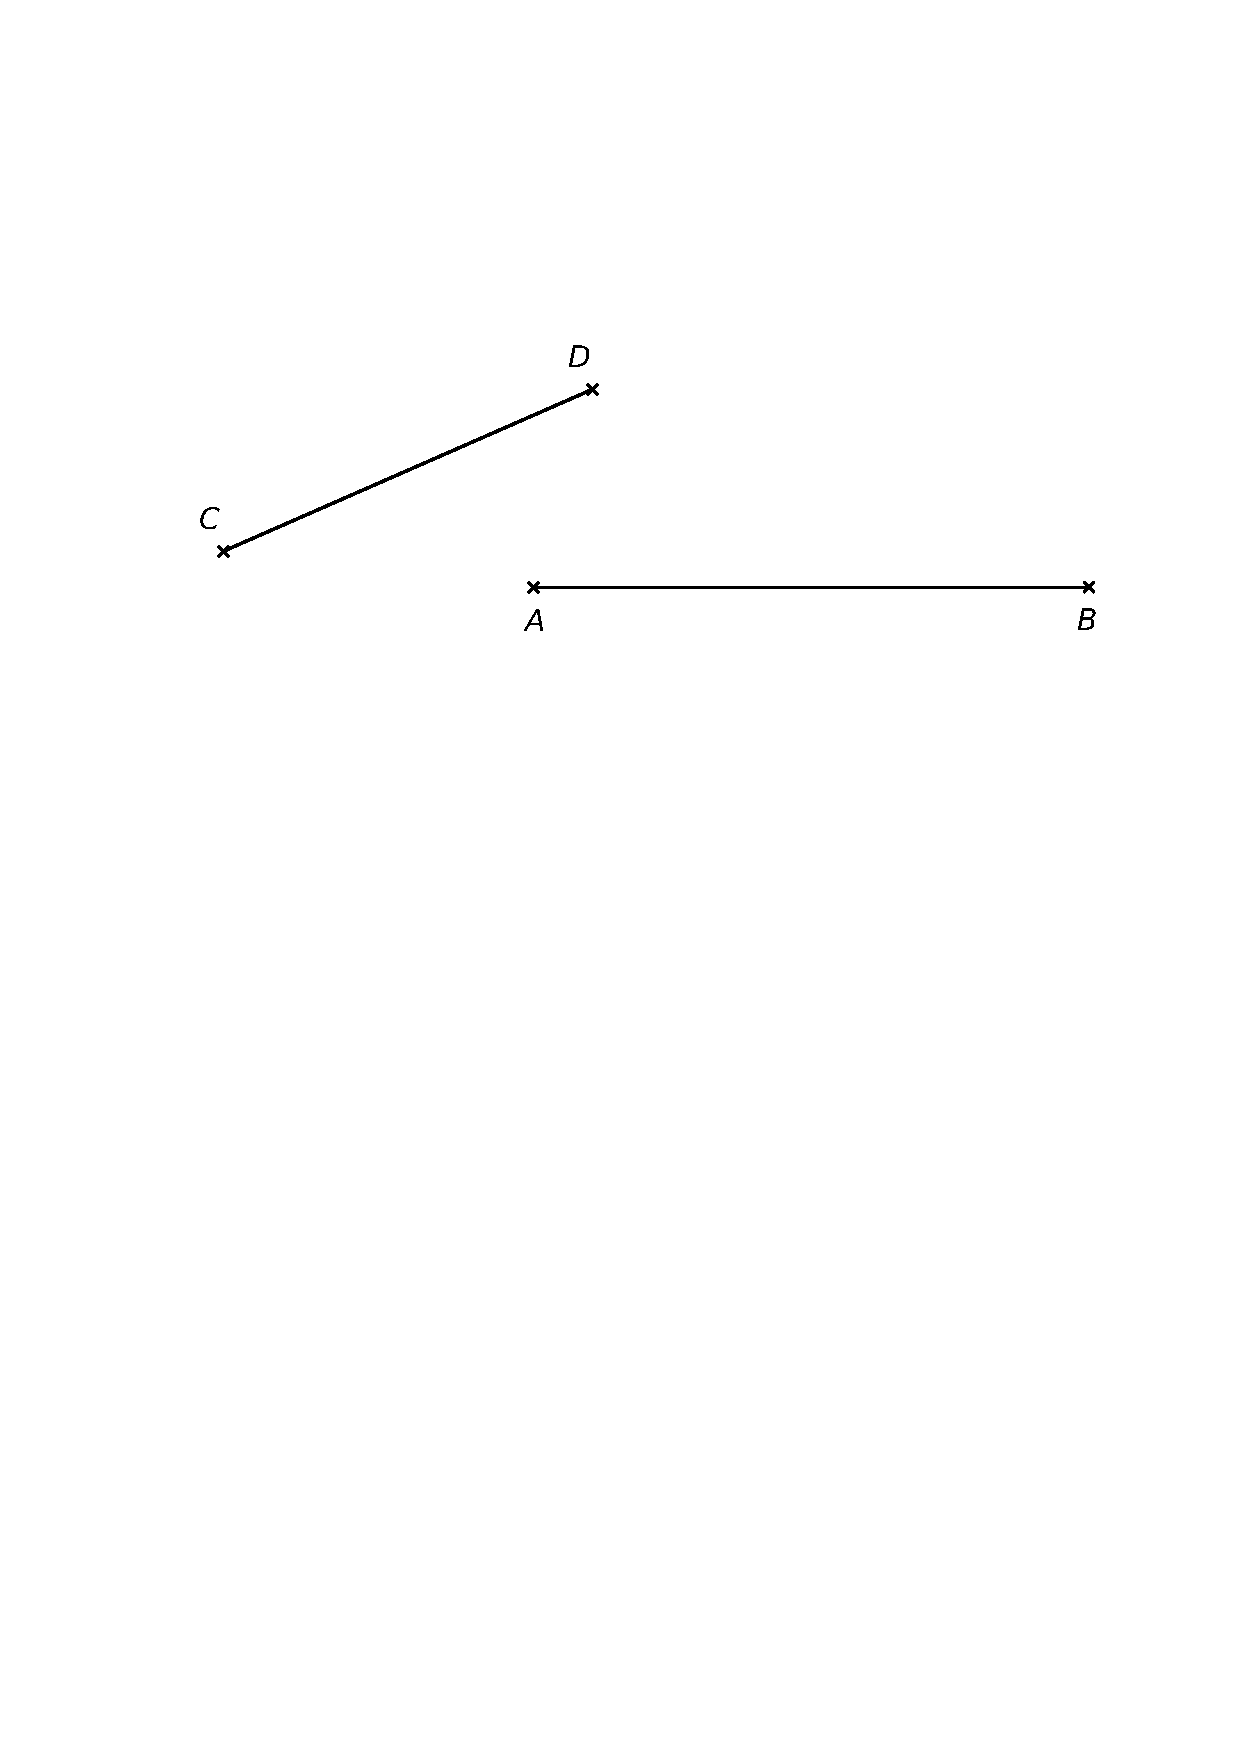
\includegraphics[scale=1]{media/es-10/12-8}
\end{center}
\vspace{2cm}

%\psset{xunit=1cm,yunit=1cm,algebraic=true,dimen=middle,dotstyle=o,dotsize=5pt 0,linewidth=2pt,arrowsize=3pt 2,arrowinset=0.25}
%\begin{pspicture*}(8.39,-3.99)(20.59,-1.11)
%\psline[linewidth=2pt](9.83,-2.17)(11.83,-2.17)
%\psline[linewidth=2pt](13.91,-3.29)(17.91,-1.29)
%\begin{scriptsize}
%
%
%\psdots[dotstyle=x](9.83,-2.17)
%\rput[bl](9.91,-1.97){$E$}
%\psdots[dotstyle=x](11.83,-2.17)
%\rput[bl](11.91,-1.97){$F$}
%\psdots[dotstyle=x](13.91,-3.29)
%\rput[bl](13.99,-3.09){$G$}
%\psdots[dotstyle=x](17.91,-1.29)
%\rput[bl](17.99,-1.5){$J$}
%\end{scriptsize}
%\end{pspicture*}
%\vspace{2cm}
}
{1}
\end{exop}


\begin{exop}
{Dominique souhaite placer une table (dénotée par un point $T$) à égale distance de la fenêtre $F$ et de la porte $P$ dans la pièce schématisée ci-dessous. Trace sur la figure où elle pourrait la placer. Est-ce la seule possibilité~?

\begin{center}
	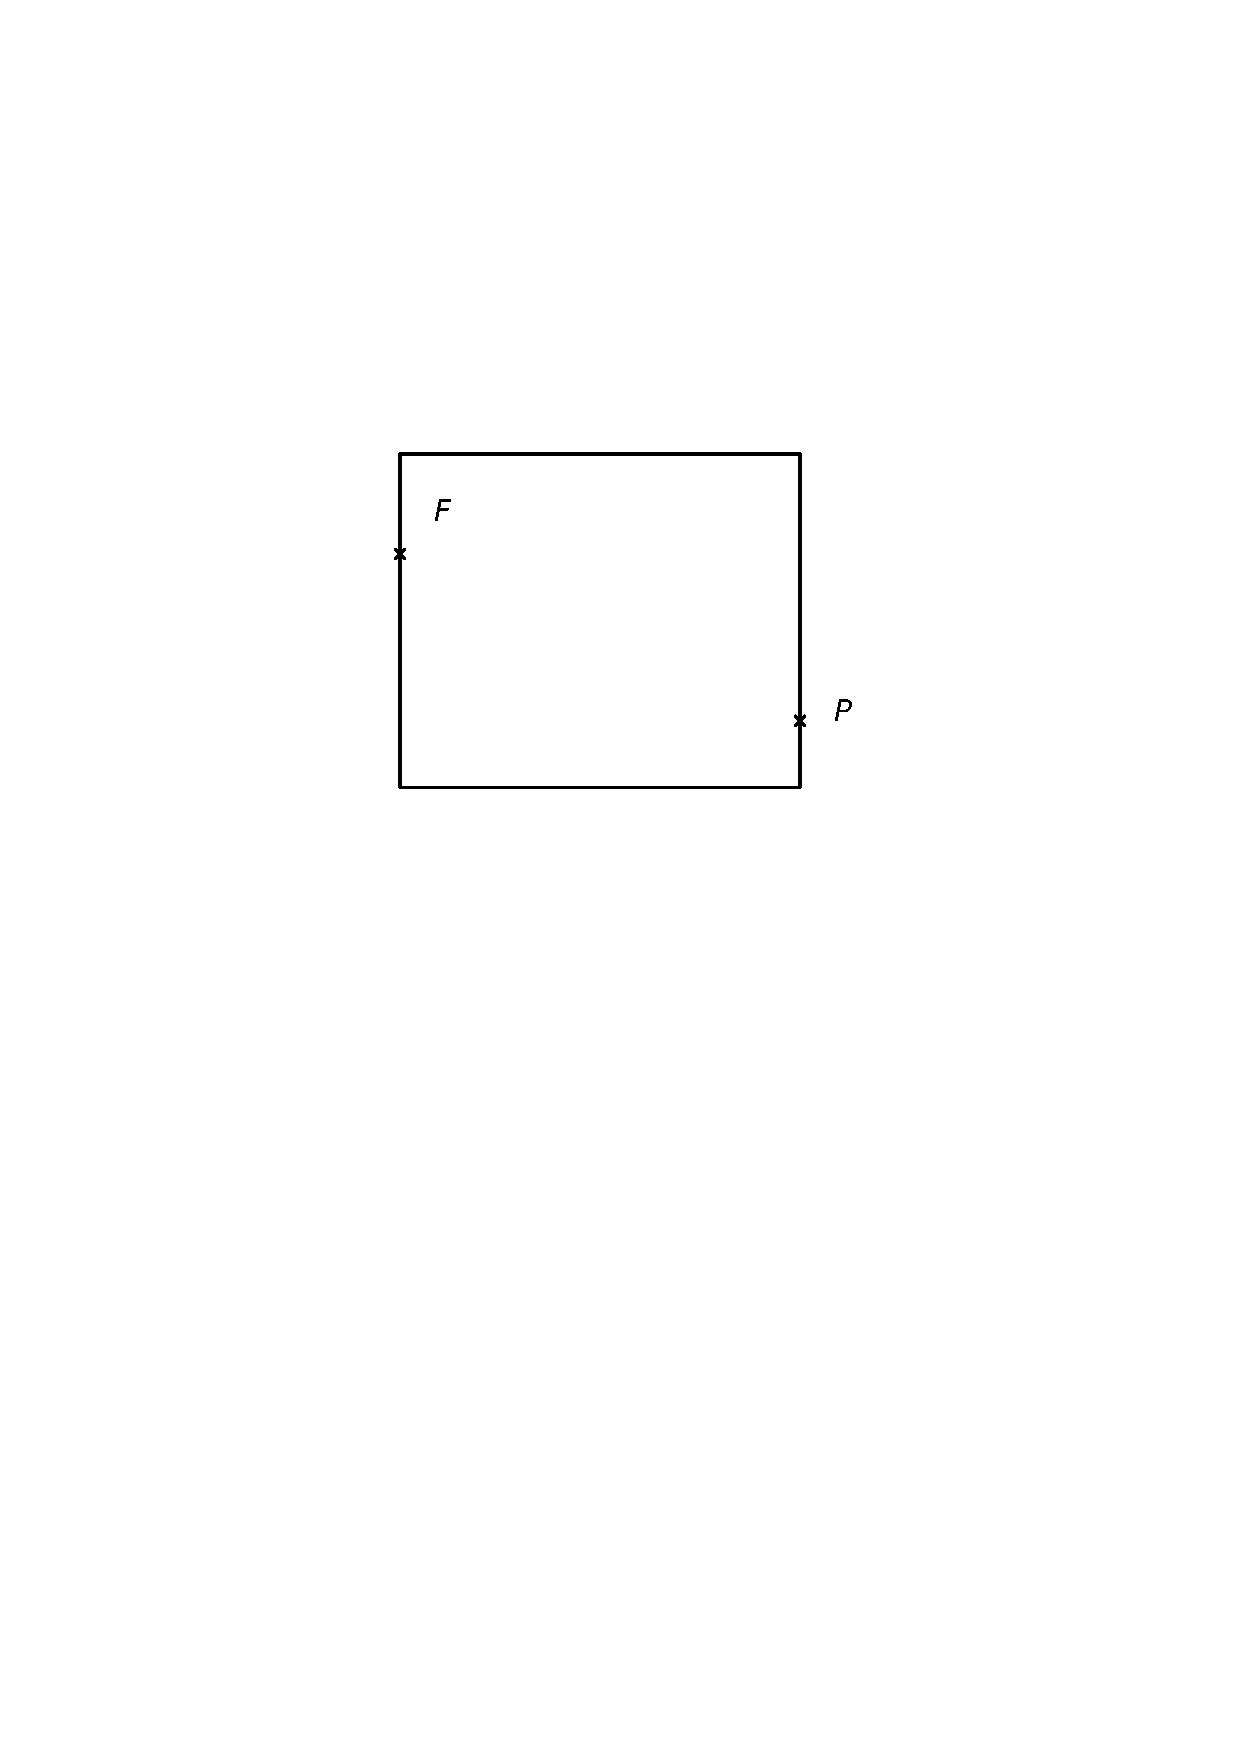
\includegraphics[scale=1]{media/es-10/12-9}
\end{center}
%\psset{xunit=1cm,yunit=1cm,algebraic=true,dimen=middle,dotstyle=o,dotsize=5pt 0,linewidth=2pt,arrowsize=3pt 2,arrowinset=0.25}
%\begin{pspicture*}(-3.63,-4.08)(9.99,1.44)
%\begin{scriptsize}
%\psdots[dotstyle=x](-2.13,-1.2)
%\rput[bl](-2.05,-1){$F$}
%\psdots[dotstyle=x](7.37,-2.68)
%\rput[bl](7.45,-2.48){$P$}
%\end{scriptsize}
%\end{pspicture*}
}
{2}
\end{exop}
\begin{exof}{ES23}{114}{1}
\end{exof}

\begin{exof}{ES24}{115}{1}
\end{exof}

%\begin{resolu}{Les bissectrices}
%{Trace la bissectrice de l'angle $\widehat{ABC}$
%\vspace{3cm}
%\begin{center}
%\begin{tikzpicture}
%   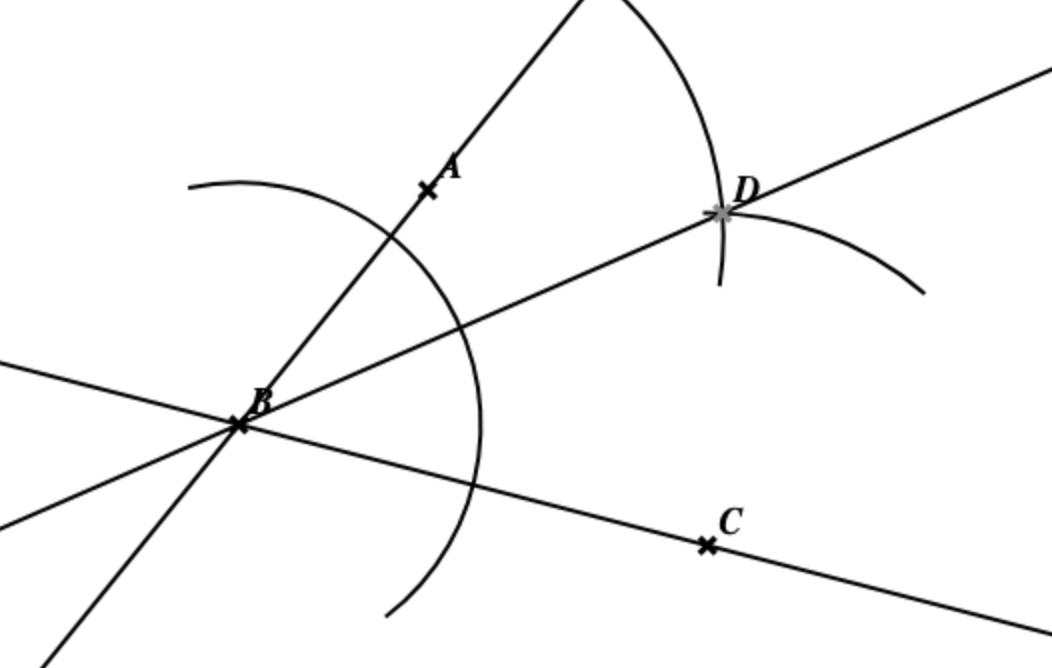
\includegraphics [scale=0.4]{media/es-10/bissectrice.png} [!h]
%\end{tikzpicture}
%\end{center}
%{\color{blue} A l'aide des traits de construction (arcs de cercles), on obtient le point D. Pour tracer la bissectrice, on relie le sommet B au point D.}
%}
%{1}
%\end{resolu}

\begin{exop}
{Trace la bissectrice de l'angle $\widehat{fOg}$.

\begin{center}
	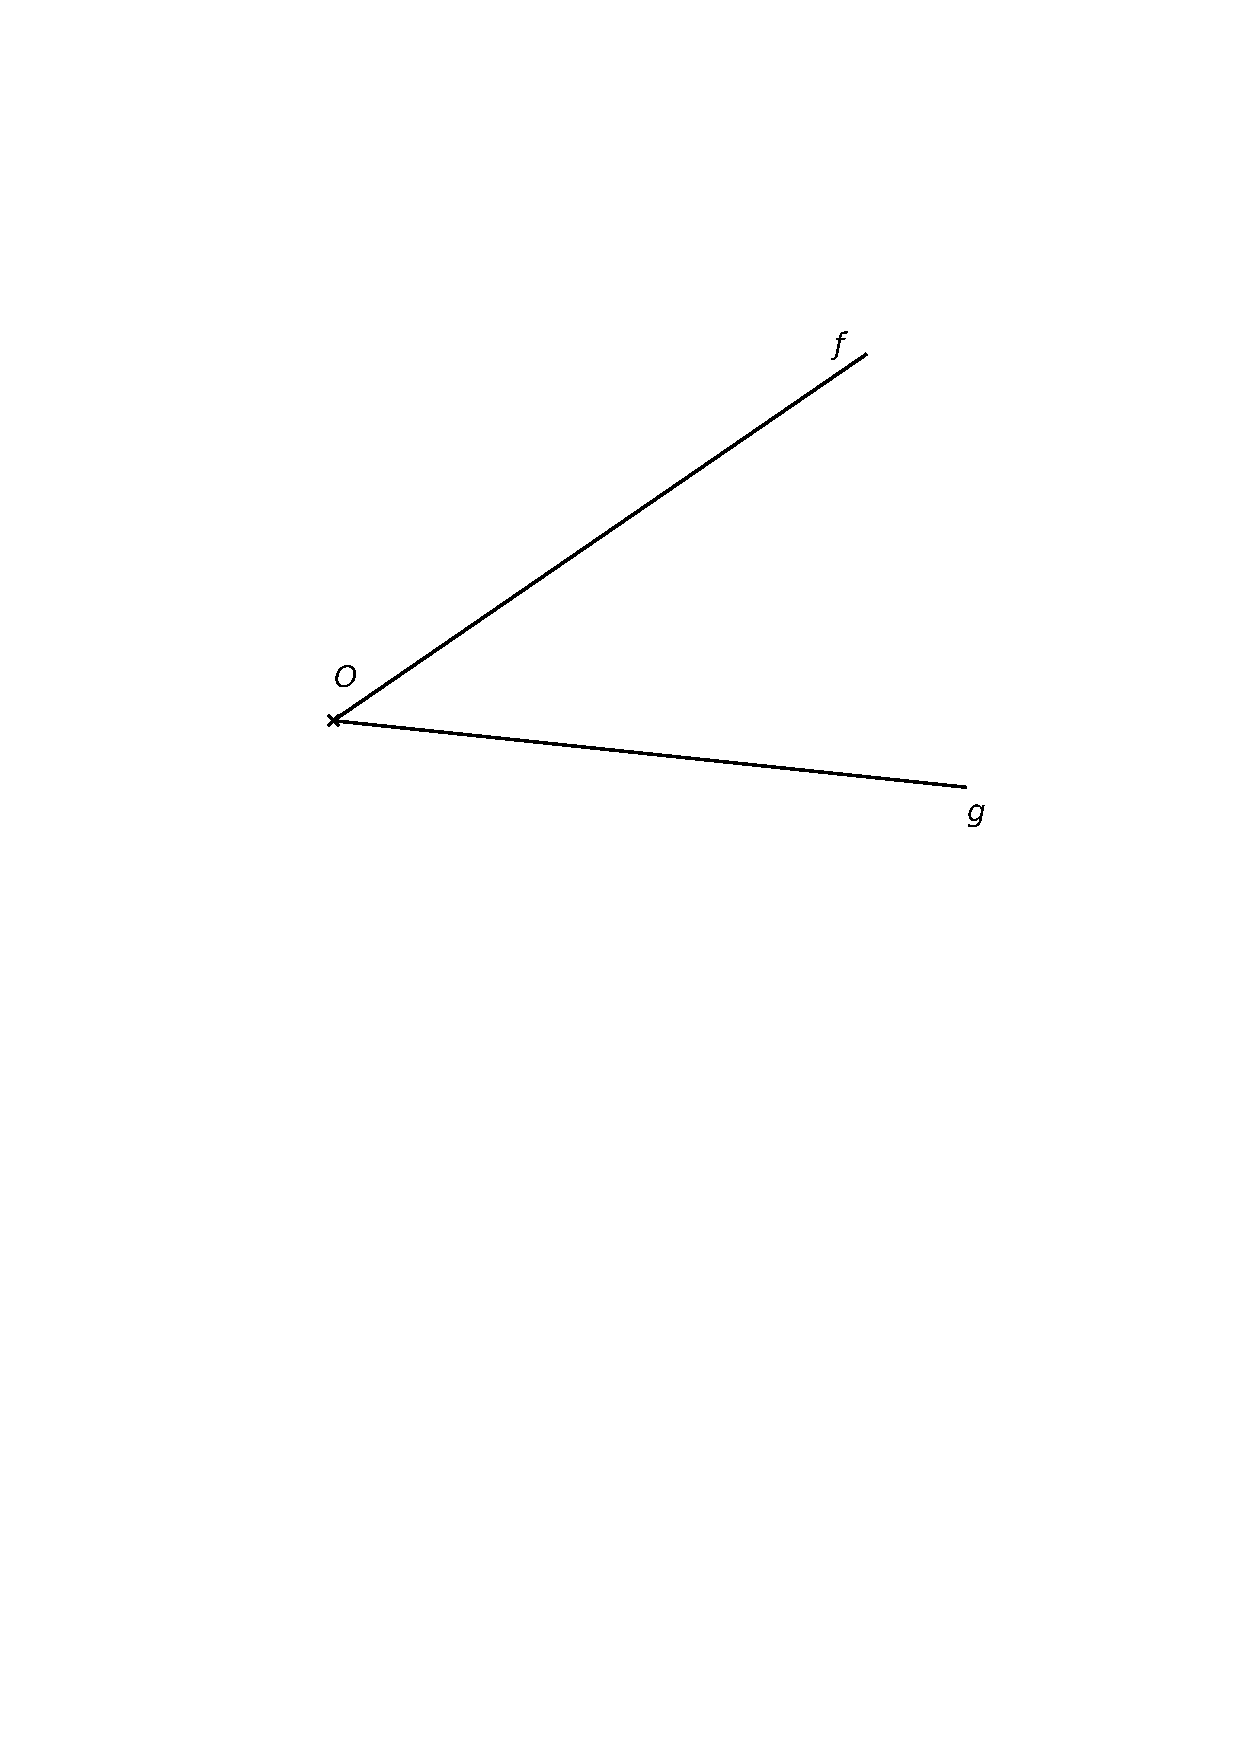
\includegraphics[scale=1]{media/es-10/12-10}
\end{center}
\vspace{1cm}
%\begin{center}
%
%\psset{xunit=1cm,yunit=1cm,algebraic=true,dimen=middle,dotstyle=o,dotsize=5pt 0,linewidth=2pt,arrowsize=3pt 2,arrowinset=0.25}
%\begin{pspicture*}(-5.54,-2.76)(5.54,2.76)
%\psplot[linewidth=2pt]{-5.54}{5.54}{(-9.5464-2.96*x)/-3.06}
%\psplot[linewidth=2pt]{-5.54}{5.54}{(-6.288-1.24*x)/3.92}
%\begin{scriptsize}
%\rput[bl](-5.38,-1.86){$f$}
%\rput[bl](-5.16,0.26){$g$}
%\psdots[dotsize=4pt 0,dotstyle=x,linecolor=darkgray](-3.68,-0.44)
%\rput[bl](-3.7,-0.25){\darkgray{$O$}}
%\end{scriptsize}
%\end{pspicture*}
%\end{center}
}
{1}
\end{exop}

\begin{exop}
{Trace la bissectrice de l'angle $\widehat{fOg}$.
\begin{center}
	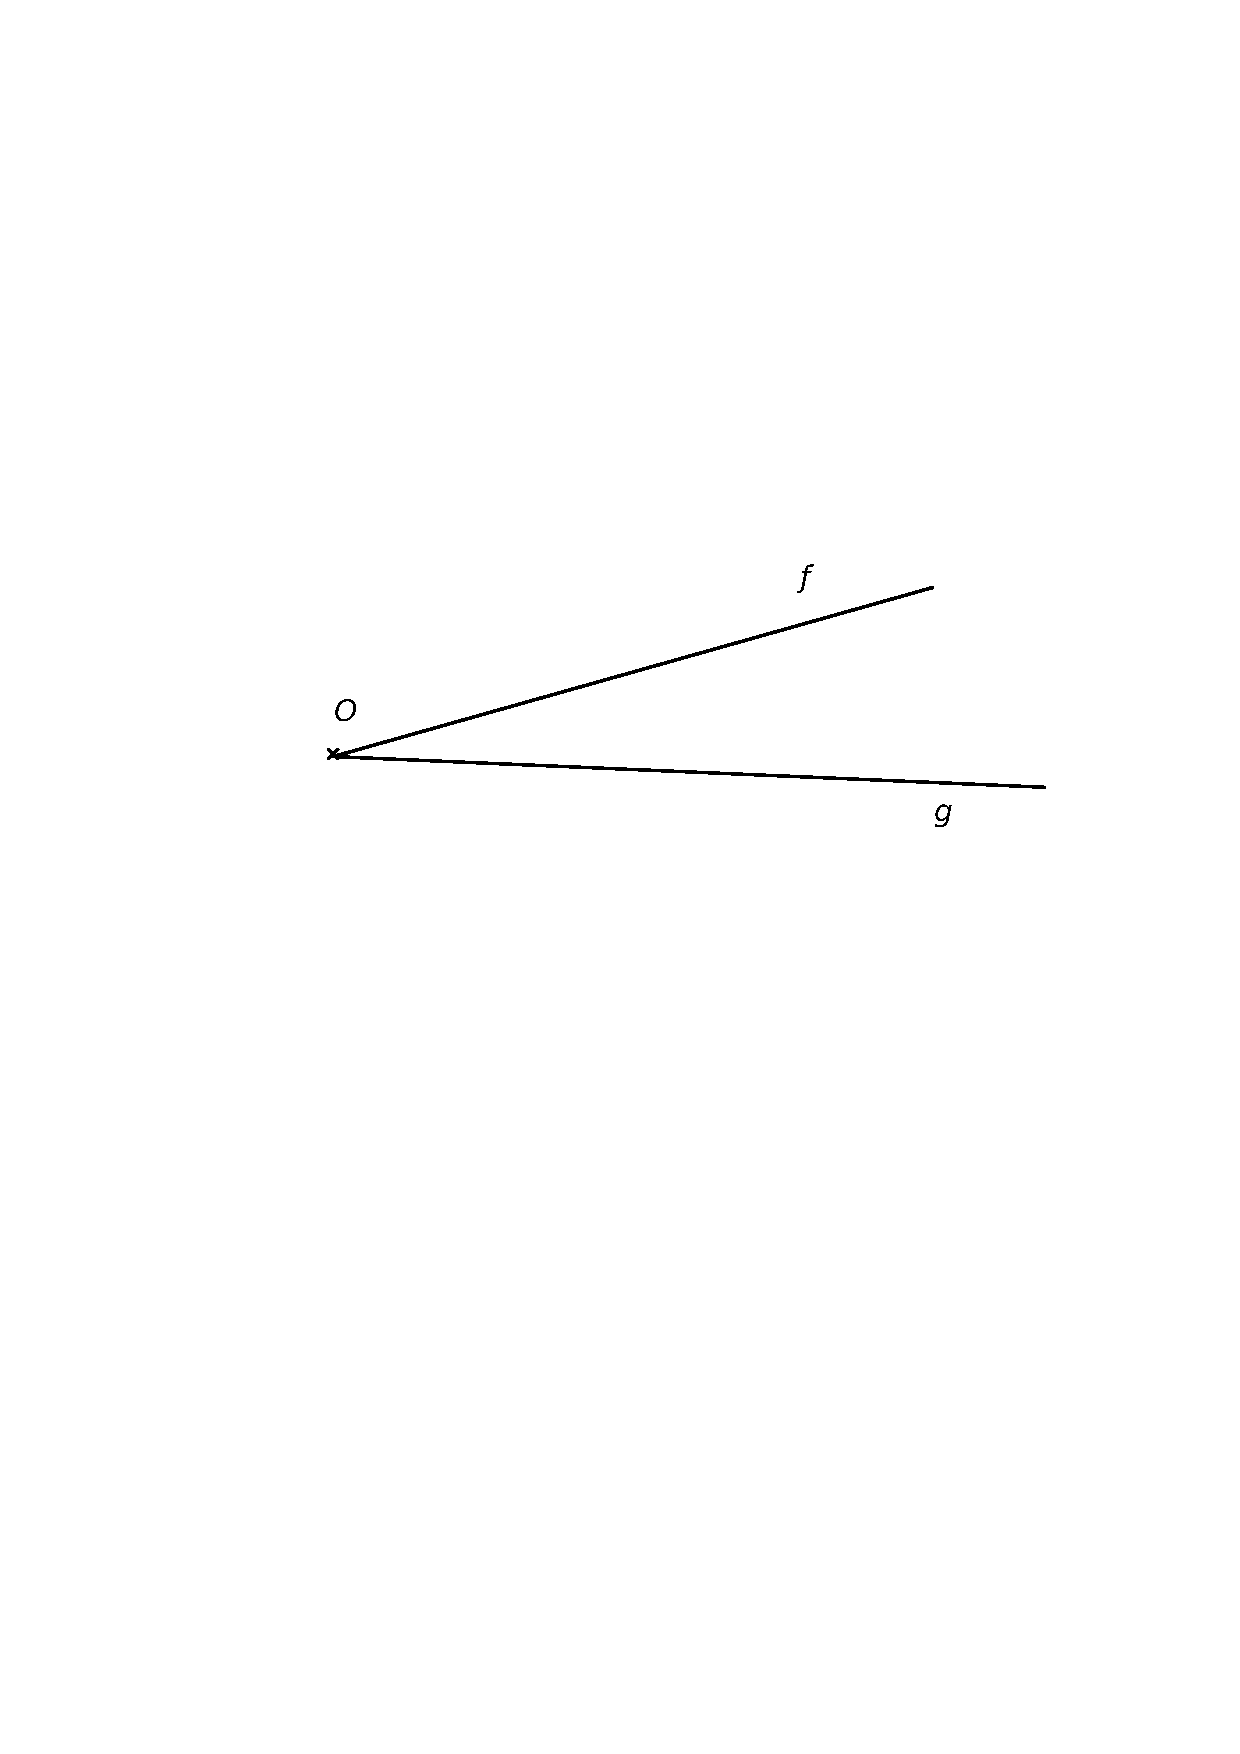
\includegraphics[scale=1]{media/es-10/12-11}
\end{center}
\vspace{1cm}
%\begin{center}
%
%\psset{xunit=1cm,yunit=1cm,algebraic=true,dimen=middle,dotstyle=o,dotsize=5pt 0,linewidth=2pt,arrowsize=3pt 2,arrowinset=0.25}
%\begin{pspicture*}(-5.54,-1.5)(5.54,2.76)
%\psplot[linewidth=2pt]{-5.54}{5.54}{(-6.7636-0.68*x)/-4.22}
%\psplot[linewidth=2pt]{-5.54}{5.54}{(--3.6912-0.34*x)/4.32}
%\begin{scriptsize}
%\psdots[dotstyle=x](-3.12,1.1)
%\rput[bl](-3.04,1.3){$O$}
%\rput[bl](-5.38,0.42){$f$}
%\rput[bl](-5.36,1.52){$g$}
%\end{scriptsize}
%\end{pspicture*}
%\end{center}
}
{1}
\end{exop}

\begin{exop}
{Sur la figure ci-dessous, 
\begin{tasks}(1)
	\task Place le point $P$ équidistant à $A$ et $B$ et aux droites $f$ et $g$.
	\task Place le point $Q$ équidistant à $A$ et $C$ et aux droites $f$ et $g$.
\end{tasks}

\begin{center}
	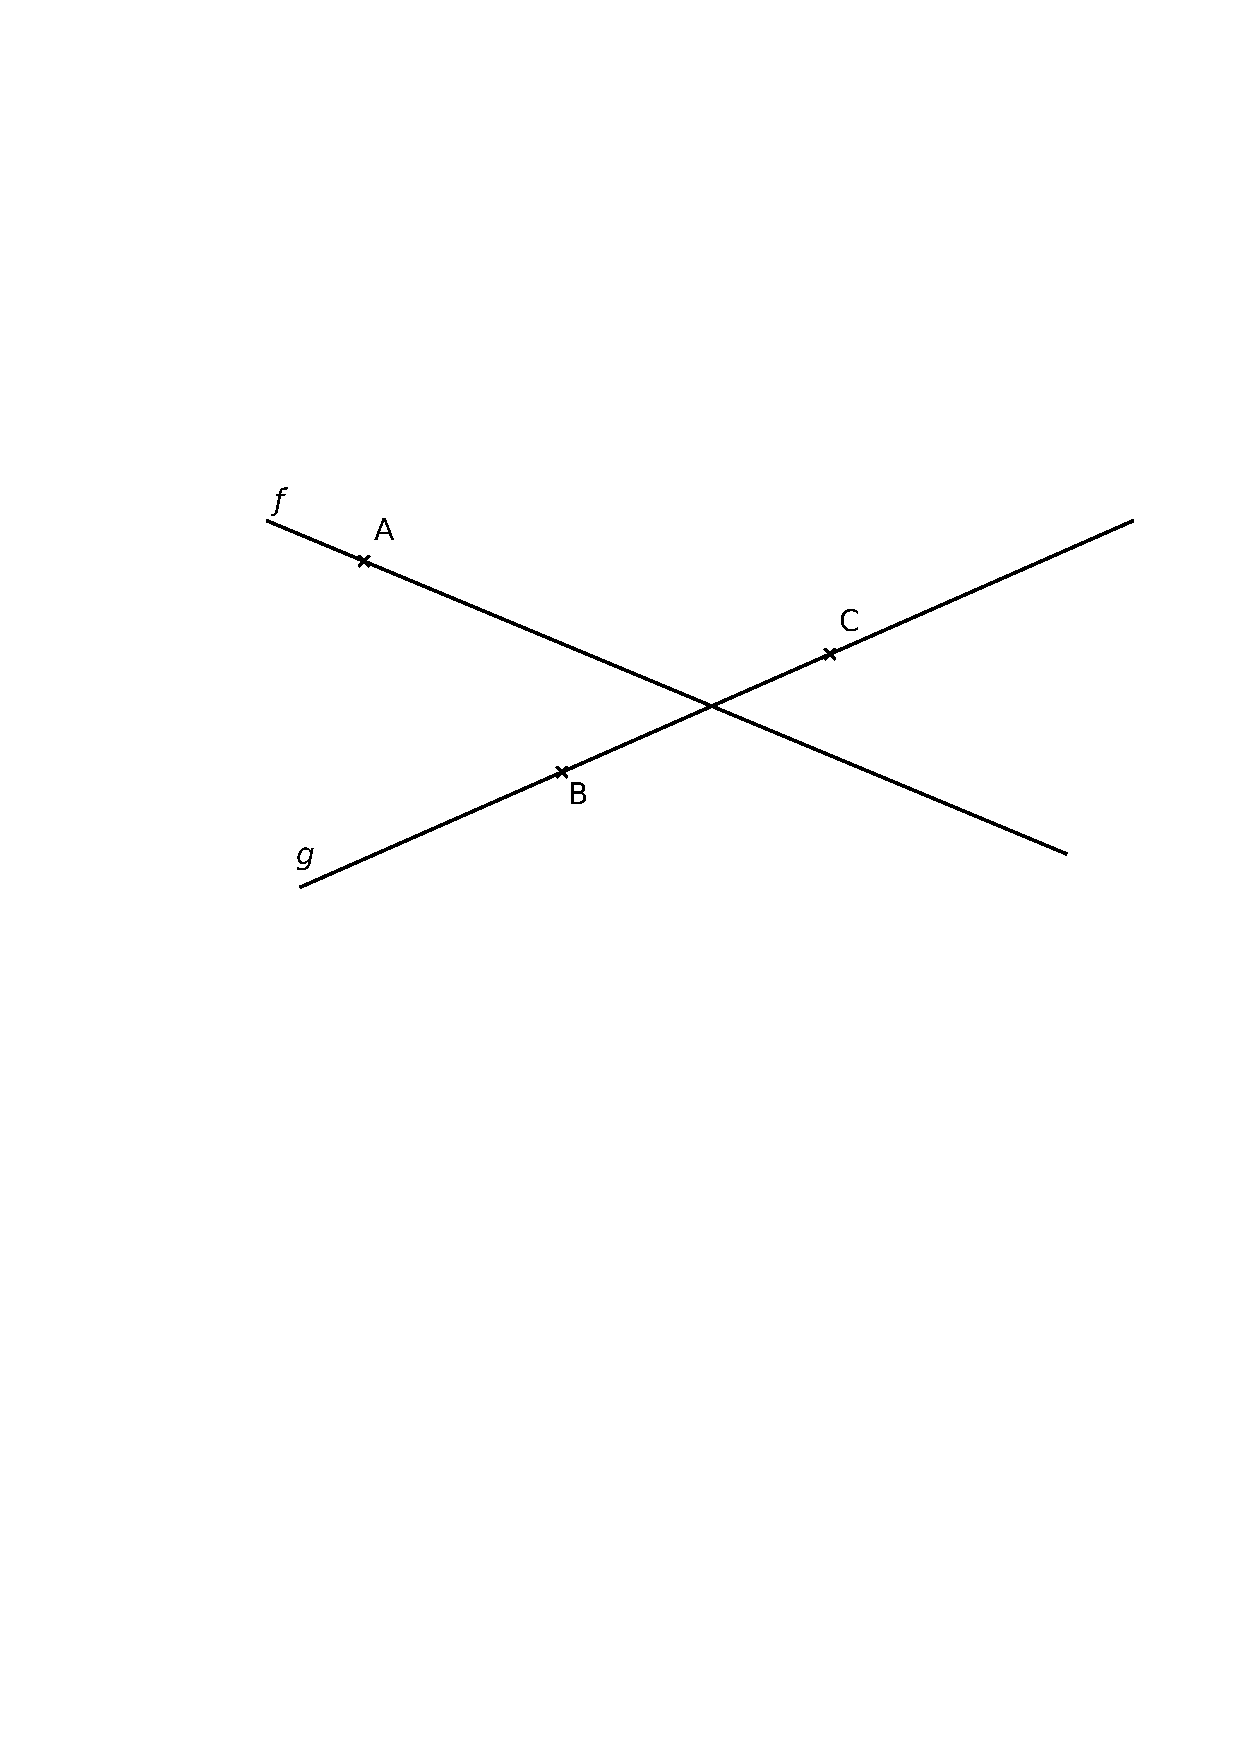
\includegraphics[scale=1]{media/es-10/12-12}
\end{center}
%\begin{center}
%
%\psset{xunit=1cm,yunit=1cm,algebraic=true,dimen=middle,dotstyle=o,dotsize=5pt 0,linewidth=2pt,arrowsize=3pt 2,arrowinset=0.25}
%\begin{pspicture*}(-3.56,-5.28)(9.04,3.46)
%\psplot[linewidth=2pt]{-3.56}{9.04}{(--7.5564-3.14*x)/8.1}
%\psplot[linewidth=2pt]{-3.56}{9.04}{(--6.6564-3.04*x)/-9.66}
%\begin{scriptsize}
%\psdots[dotstyle=x](-2.34,1.84)
%\rput[bl](-2.26,2.04){$A$}
%\psdots[dotstyle=x](5.76,-1.3)
%\rput[bl](5.84,-1.1){$B$}
%\rput[bl](-3.4,1.92){$f$}
%\psdots[dotstyle=x](8.1,1.86)
%\rput[bl](8.18,2.06){$C$}
%\psdots[dotstyle=x](-1.56,-1.18)
%\rput[bl](-1.48,-0.98){$D$}
%\rput[bl](-3.4,-1.58){$g$}
%\end{scriptsize}
%\end{pspicture*}
%\end{center}
}
{2}
\end{exop}
\begin{exof}{ES26}{116}{1}
\end{exof}

\begin{exol}{ES32}{100}{1}
\end{exol}

\begin{exol}{ES33}{101}{1}
\end{exol}

\begin{exof}{ES25}{116}{1}
\end{exof}

\begin{exof}{ES28}{118}{1}
\end{exof}

\begin{exof}{ES30}{118}{1}
\end{exof}




%\begin{exop}
%{Sur la figure ci-dessous, trace le point Q à $1,5 cm$ du point C, à $2 cm$ du point B et équidistant des droites f et g.

%\begin{center}
%    
%\psset{xunit=1cm,yunit=1cm,algebraic=true,dimen=middle,dotstyle=o,dotsize=5pt 0,linewidth=2pt,arrowsize=3pt 2,arrowinset=0.25}
%\begin{pspicture*}(-3.56,-5.28)(9.04,3.46)
%\psplot[linewidth=2pt]{-3.56}{9.04}{(--7.5564-3.14*x)/8.1}
%\psplot[linewidth=2pt]{-3.56}{9.04}{(--6.6564-3.04*x)/-9.66}
%\begin{scriptsize}
%\psdots[dotstyle=x](-2.34,1.84)
%\rput[bl](-2.26,2.04){$A$}
%\psdots[dotstyle=x](5.76,-1.3)
%\rput[bl](5.84,-1.1){$B$}
%\rput[bl](-3.4,1.92){$f$}
%\psdots[dotstyle=x](8.1,1.86)
%\rput[bl](8.18,2.06){$C$}
%\psdots[dotstyle=x](-1.56,-1.18)
%\rput[bl](-1.48,-0.98){$D$}
%\rput[bl](-3.4,-1.58){$g$}
%\end{scriptsize}
%\end{pspicture*}
%\end{center}
%}
%{2}
%\end{exop}

\begin{exol}{ES36}{102}{1}
\end{exol}



\begin{exo}
    {Effectue les constructions suivantes dans ton cahier:
    \begin{tasks}(1)
	    \task Trace un cercle de centre $O$ et de rayon \tunit{3}{\cm}.
	\task Place un point A sur ce cercle, puis trace une corde $[AB]$ telles que $[AB]$ mesure \tunit{1,6}{\cm}.
        \task Trace la médiatrice de $[AB]$. Soient $C$ et $D$ les intersections entre la médiatrice et le cercle.
        \task Soit $\widehat{AOC}$, trace la bissectrice de cet angle.
    \end{tasks} 
    }
 {2}   
\end{exo}

\begin{exol}{ES38}{103}{2}
\end{exol}

\begin{exol}{ES39}{103}{1}
\end{exol}

\begin{exol}{ES37}{102}{1}
\end{exol}

\begin{exol}{ES40}{104}{2}
\end{exol}

\begin{FLP}{119}{1}
\end{FLP}



\end{document}
